\subsection{Product perspective}
\subsubsection{Scenarios}
\textbf{Sign-up} \\ [5pt]
Cyclist John opens the platform for the first time and clicks on the \textit{Sign Up} option to create a new account. The system shows a form where John inserts his name, his email and chooses a password to authenticate the next times. After that, John clicks the \textit{Sign Up} button and is shown the home page of the platform.\\[8pt]
\textbf{Login} \\ [5pt]
Cyclist John has already registered on the platform and wants to authenticate. He clicks on \textit{Login} option, the system shows a form where John inserts his credentials, and then clicks the button \textit{Login}. After that, the home page of the platform is shown.\\[8pt]
\textbf{Access as a Guest}\\ [5pt]
Guest Bob wants to visualize the paths available on the platform without performing the Login. He opens the platform and clicks on \textit{Continue as Guest}. After that, the home page of the platform is shown and it is the only interactive screen.\\[8pt]
\textbf{Account management} \\[5pt]
To view his personal account, John has to click the \textit{Account} button. From this screen, he can access all the statistics related to his activities. From the account screen, John can also edit his account by clicking on \textit{Edit Account}. 
\\[8pt]
\textbf{Visualize the personal inventory} \\[5pt] Cyclist John wants to view his inventory, so he clicks the \textit{Inventory} button. This allows the cyclist to view to all his ride performances. By clicking on a specific path, he can then view its detailed statistics and the related routes 
\\[8pt]
\textbf{Manage a route} \\[5pt]
After having visualized the inventory, Cyclist John wants to manage his route. He clicks on the route to expand the view and visualize the management buttons.
\begin{itemize}
    \item Pressing the \textit{Publish} button, John shares the route with the community. As a consequence, the same button when pressed becomes the dual version \textit{Unpublish}.
    \item Pressing the \textit{Delete} button, John removes his route from the related path and from his inventory.
\end{itemize} 
\textbf{Route creation} \\[5pt]
Cyclist John clicks the  \textit{Create} button to access the Route creation screen.
\begin{itemize}
    \item \textbf{Manual Route creation:}
Cyclist John begins the process by clicking the \textit{Start} button in the manual route creation section. He first enters the starting point, then adds all the way points, meaning the individual roads he travels along, and finally specifies the end point.
Once this step is completed, he proceeds to the next screen, where he provides a description, the duration, and the status.
To finish, he saves the route by clicking the \textit{Save} button.
    \item \textbf{Automatic Route creation:}
Cyclist John begins by clicking the \textit{Start tracking} button in the automatic route creation section. Then he visualizes a new screen, where he clicks \textit{Start tracking} again. From that moment, the system starts to automatically track the cyclist movements. Once the ride is completed, John stops the tracking, reviews the automatically generated route, and finalizes by saving it.
\end{itemize}
\textbf{Route Planning} \\[5pt]
To plan a new route, the cyclist John clicks the \textit{Home} button and enters the starting point and the destination of the path he intends to follow. John may also choose to specify a tolerance in kilometers.
He then presses \textit{Search paths} to view all the routes that match his criteria. \\[8pt]
\textbf{Visualize a path from the search results} \\ [5pt]
By selecting a path, John can view the map, the average time, the distance, the status, and the score associated with that path. Moreover, similar routes will be displayed in the section below. \\[8pt]
\textbf{Navigation} \\ [5pt]
User Jade visualizes a path and clicks the button \textit{Start Navigation}. 
\\The platform provides Jade with a navigation map to guide her along the selected path. When the end point is reached, a \textit{Path completed} message is displayed.
\begin{itemize}
    \item If Jade is a cyclist in the next screen she provides all the details of the routes and proceeds to save the route in his inventory by clicking the \textit{save} button.
    \item If Jade is a guest the system shows a message "You have to login to save a route".
\end{itemize}
\subsubsection{Domain Class Diagrams}
\begin{figure}[H]
\centering
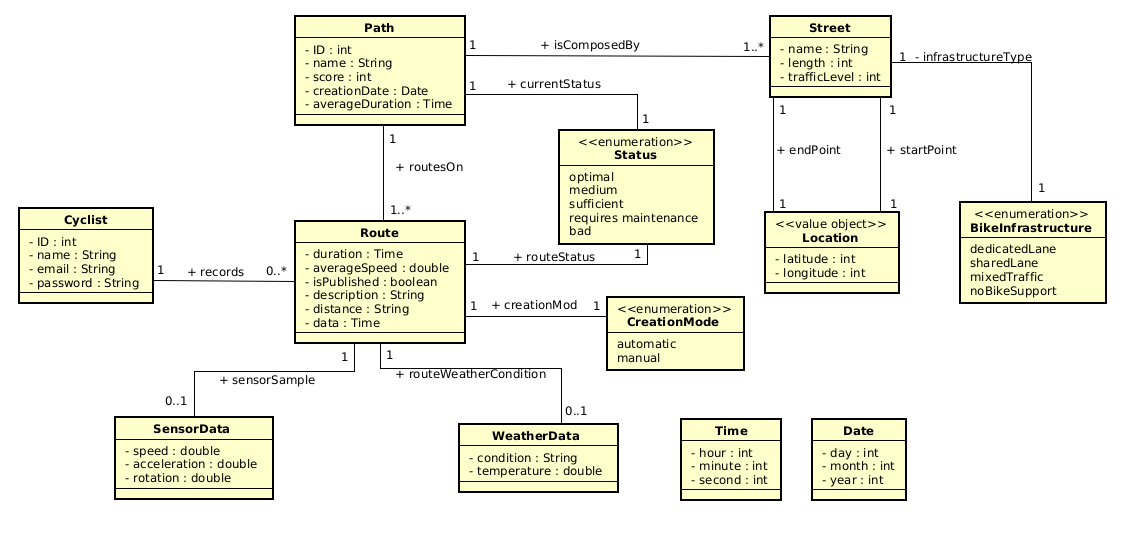
\includegraphics[width=1\textwidth]{Images/ClassDiagram.png}
\caption{\label{fig:metamodel2}Domain Class Diagram}
\end{figure}
This is the class diagram of BBP. The system can also be used by guest user but it is not necessary store any information about them because guests can only view content but can not interact with the system by creating and managing their routes. All the other users of the app are registered and they are described by the \textbf{Cyclist class}. The classes Path and Route describe related concepts but they have a different role in the application.\\
\textbf{Path class}, a path is the most general description of a set of streets, \textbf{Street class}. The streets of the paths can be collected automatically by the mobile device (and then confirmed by the cyclist) or directly entered manually by the Cyclist, this distinction is modeled by the \textbf{CreationMode enum}.
For each street it's stored not only general information but also the exact location where it starts and ends \textbf{Location valueObject} and the type of bike infrastructure \textbf{BikeInfrastructureType enum}.\\
\textbf{Route class}, a route instead represents an actual ride performed by a cyclist on a specific path. If a route is performed on a path  that is not present yet in the system, a new path will be created and that route will be set as the route that generated the path.
Each route is enriched with sensors data \textbf{ SensorData class} and with weather condition, \textbf{WeatherCondition class}.\\
\textbf{Status enum}, the status represents the quality of the road surface when a route is recorded or more broadly the current condition of a path, updated using the most recent information available in the system.
\subsubsection{State Diagrams}
\begin{figure}[H]
\centering
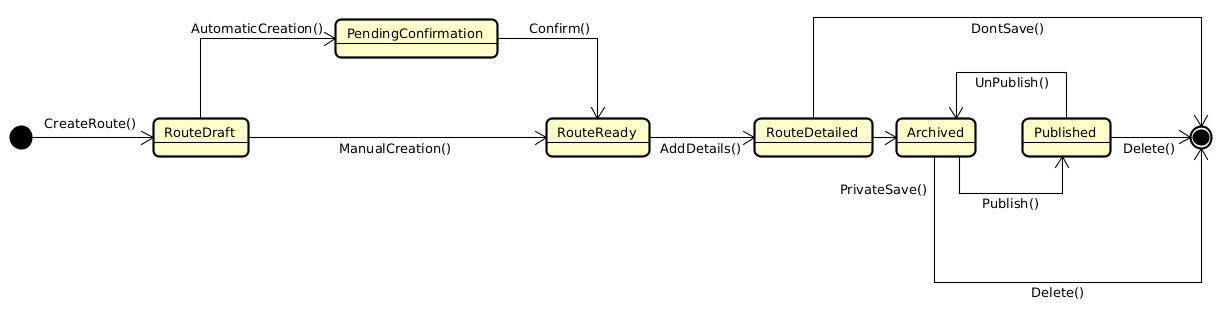
\includegraphics[width=\textwidth]{Images/RouteDiagramState.png}
\caption{\label{fig:metamodel2} State Diagram - Route creation}
\end{figure}
The state diagram in figure describes the lifecycle of a route from its creation to its publication, archiving, or deletion. The process starts from the initial state, where the \textit{CreateRoute()} event moves the route into the \textbf{RouteDraft} state, representing a newly created draft. From this state, two alternative ways are possible:
\begin{itemize}
    \item \textit{AutomaticCreation()} leads to the \textbf{PendingConfirmation} state until the Cyclist does not confirm the information collected. Once the \textit{Confirm()} event occurs, the state changes into \textbf{RouteReady} state
    \item \textit{ManualCreation()} leads directly to the \textbf{RouteReady} state, skipping the confirmation phase
\end{itemize}
The \textbf{RouteReady} state indicates that the route is prepared but not yet complete, because the details are still missing. The \textit{AddDetails()} event makes the transition to the \textbf{RouteDetailed} state happen, where all required details have been added. From this state, the route enters a region that manages its visibility and persistence:
\begin{itemize}
    \item With \textit{PrivateSave()}, the route is stored and goes to the \textbf{Archived} state.
    \item The \textit{DontSave()} event allows the Cyclist to discard the route, leading directly to the end of the lifecycle.
    \item From \textbf{Archived}, the \textit{Publish()} event allows the route to be made public, transitioning it to the \textbf{Published} state. Dually, from \textbf{Published} state, the \textit{Unpublish()} event moves the route back to the \textbf{Archived} state.
\end{itemize}
Finally, from both the \textbf{Archived} and \textbf{Published} states, the \textit{Delete()} event transitions the route to the final state, representing its permanent removal.
\subsection{Product Functions}
\subsubsection {Sing-up and login}
This feature allows cyclists to access  their personal account  using the authentication credentials (e-mail and password). In his personal area, the cyclist can manage his account uploading a picture or changing the credential, view the total number of routes characterized by total distance and time. Unregistered users can login as guests and can only view published routes.
\subsubsection {Route creation}
Cyclists can create new routes either manually or automatically and upload them to the platform.
In manual mode, the user has to specify each road traveled one by one; in automatic mode, instead, they start the recording and the system collects data through the device’s GPS and other sensors.
Users can also enter and share information regarding the condition of cycling routes, specifying their quality level and reporting the presence of any relevant obstacles, such as potholes or damaged sections.
A cycling route refers to a path equipped with a dedicated bike lane or an area where car traffic is limited and speed limits are compatible with the average pace of a bicycle.
Each route is later enriched by the system through the addition of various statistics, such as total distance, average speed, and other performance indicators.
When available, weather conditions retrieved from external services are also integrated.
\subsubsection {Path creation} 
A path is automatically created by the system when a cyclist records a route for which no corresponding path already exists. Once the path has been created, any new route with a similar path will be associated with that path.
\subsubsection{Manage inventory}
Cyclists can visualize their inventory filtering by published paths and by the status of the paths. Moreover it is possible to order the paths inside the inventory by: date, distance and score.
They can also see a specific route of a path and decide to publish, unpublish or delete it.
\subsubsection {Route publication}
Cyclists can choose to share one or more of the routes they have created with the community.
This operation can be easily performed from their personal inventory, where they can select the routes they wish to make public.
Once published, the route becomes visible to other cyclists on the platform and may appear in the results when users explore new paths to follow.
In this way, each cyclist contributes to enriching the library of available routes, promoting sharing and the discovery of new experiences.
\subsubsection {Route planning}
Users can search for new paths to follow within the platform by entering a starting point, a destination, and a tolerance value expressed in kilometers allowing greater flexibility in the search. 
Once these parameters are provided, the system generates a list of paths that match the given criteria.
For each path, the main information is displayed: name, distance, average time, status and score.
Users can choose an existence path and start the navigation and if they are Cyclists they may also choose to save the route in their inventory 
\subsubsection {Scoring and Ranking}
The system calculates a score for each path in order to evaluate its overall quality and its ability to satisfy the user’s request.
The score is determined by combining two main factors: the condition of the path and its effectiveness, meaning how suitable it is for connecting the user’s specified starting point and destination. The goal of the score is to allow the system to rank the different paths during searches. \\ Since path conditions may change over time, to ensure that the score remain accurate and up-to-date, when multiple users report different information about the same path, the system merges them by evaluating the date of the submitted data, giving priority to the most recent and the number of consistent reports, in order to increase the reliability of the classification.
\subsection{User characteristics}
There are two types of user that can interact with BBP and the main difference is the ownership of a personal account on the platform. In summary, registered users, called Cyclists, have full access to all features. Unregistered users, referred to as Guests, have limited access to the platform. In this document the term \textit{User} will be used referring to both Cyclist and Guest. \\Moreover there is a third actor that is the WeatherCondition service that is invoked by the system and does not interact directly with it. 
\subsubsection{Guest}
The Guest is an unregistered user who can access the platform without creating a personal account. Their interaction with the system is mainly focused on consultation: they can search for and view available bike paths, accessing their statistics, map, and status. The Guest can also benefit from the route planning system. 
\subsubsection{Cyclist}
The Cyclist is a registered user of the platform who owns a personal account. Once logged in, they can actively interact with the system, contributing to the growth of the community. \\
The Cyclist can access all features available to the Guest, as well as additional ones. In particular, the Cyclist has the possibility to create new paths either manually or automatically. After defining a path, the Cyclist can enrich it with details and evaluate with a status before saving it as a route inside his personal inventory.\\
The Cyclist therefore plays a central role within the platform: they actively contribute to the creation, evaluation, and publishing new routes, supporting the continuous improvement of the system and the expansion of the archive of paths available to all users.
\subsubsection{WeatherCondition}
The WeatherCondition is an external service used by the system to enrich routes data with information about the weather condition.
\subsection{Assumptions, dependencies and constraints}
\subsubsection{Domain Assumptions}
\begin{itemize}
 \item \textbf{D1:} The cyclist's account data is correct.
 \item \textbf{D2:} The cyclist remembers his credentials.
 \item \textbf{D3:} The cyclist manually adds a route only after actually completing it.
 \item \textbf{D4:} When creating and evaluating a route, the cyclist inputs accurate and realistic information.
 \item \textbf{D5:} Reliable meteorological information.
 \item \textbf{D6:} If cyclists use GPS, accelerometer and gyroscope we assume that they are accurate and work correctly. 
 \item \textbf{D7:} There are always paths available from point A to point B for any tollerance level.
 \item \textbf{D8:} The starting and ending point are reasonable, so that they do not necessarily require the use of other means of transportation.
 \item \textbf{D9:} All users have a reliable internet connection.
\end{itemize}